\chapter{Conclusions, major problems and future work}
This chapter will conclude the thesis, recapitulate the most important implications coming with a tool like COOP, discuss it's greatest weaknesses and shortcomings and will evaluate whether or not the author thinks that automated OOP to DoD transformation tools are a viable approach in general.

\section{Future Work}\label{future_work}
There are numerous problems coming with a performance optimization approach like COOP. Some of them were already discussed in the previous sections as we solved them or found approximations that suffice a solution. In this section we will introduce some complications, that will dismiss COOP as a viable option as it is but could conceptually be solved in future work.

\subsection{Language feature coverage and situational variety}
First of all making a tool like COOP understand all kinds of language features there are, is conceptually not necessarily difficult but a lot of work. During development most of the work was adapting code to yet another language feature that came up in a new iteration of a test source-file.\\
For example right now templates are not supported, also even just multi-variable declarations are unsupported. Not because multi-variable declarations would be hard to integrate but at some point it became clear, that focusing on language compliance is a time consuming rat hole. Especially in the beginning practically each new test file will reveal another feature or situation, that needs to be handled individually. Also while the LibTooling API is tremendously helpful it also still bears some bugs that require creative workarounds.

\subsection{Hidden field usages}\label{hidden_field_usages}
\begin{wrapfigure}[5]{r}{0.4\textwidth}
\vspace{-20pt}
\begin{lstlisting}[language=C++,name={Simple example of how to hide a field usage from the LibTooling API},label={hidden_field_usage}]
MyRecord mr;
some_function(&mr.int_field);
\end{lstlisting}
\end{wrapfigure}
The foundation of our static analysis was on the one hand to identify the records in a project as well as their respective fields. On the other hand the most important information considering our Hot/Cold split were the field usages. The LibTooling environment and especially the AST matchers provide excellent methods to filter those \textit{clang::MemberExpr} member expressions. This way we can assemble detailed charts on what is used where and by what. When given this information we can pass it to our metrics and heuristics to reason about a fields weighting. This whole process is corrupted when there are field usages, that we can't recognize as such.\\
In \refcode{hidden_field_usage} we invoke \textit{some\_function} that takes an int pointer as an argument with the address of our custom record's \textit{int\_field} field. At first glance this might be harmless, as the \textit{mr.int\_field} member usage is correctly registered by our AST matchers, however that function could invoke numerous other functions running an arbitrary amount of loops and recursion. Each consecutive use of that particular int would by our means represent a field usage however Clang won't recognize it as one.\\\\
To fix this we could rely on further static analysis to trace member usages of this kind. Whenever we find a function, that is invoked with a field for a parameter we would need to treat this function similarly to how we treat functions, that directly use instances of our records and more specifically treat that variable as a field usage for the functions scope, as well as for all functions, that are in turn invoked as well.

\subsection{False Positives}\label{false_positives}
COOP analyzes all records that are found in the given source files and provide a definition. While some records are utilized with access patterns, that allow for optimization potential using a Hot/Cold split, others are not. As of now COOP is not smart enough to recognize for example a singleton pattern or really any kind of factory pattern. So while the single instance of such a record might appear on several loops it won't have the effect on the cache COOP anticipates.\\
Right now COOP would ask the user before attempting an automated split including a user provided estimation of how many instances should be anticipated so externalizing the singleton's cold fields will not harm the instance or the systems performance, however it is an indicator, that false positives exist.\\
As long as our heuristic provides true statements about a record's 'splitability' we don't need to fear splitting it. The obtained improvements will just be so insignificant that it won't really matter. What we do need to be careful about are further changes and implementations, as those would need to consider the possibility that we are handling false positives.\\\\
On the other hand in our measurements we clearly determined that we are perfectly able to confuse COOP due to its inability of branch prediction. \Refsec{testing_oop} showed that COOP would blindly identify an exemplary particle record as a split candidate because it provided code that would results in domain heavy profiles yet those very code segments were positioned in control flow statements.\\
The resulting 'optimization' proved to be beneficial as long as (and only if) all existing particles actually performed those domain specific computations.\\
Further static analysis could reveal code segments as situational and weight them differently but ultimately, as e.g. particle amounts can vary entirely dependent on an in game situation there is no way of actually making a safe assumption about those code segments.\\
Profile guided optimizations (PGO) might come closest to providing accurate meta data for those entities but whether or not PGO is an appropriate measure also depends on the target programs purpose. Performing automated splits on records can to a certain extend predictably influence a class in a positive way, but this shows, that even with given theoretically sophisticated static analysis or PGO we can't make reliable predictions as soon as we are dealing with purely run-time dependent properties. This conceptually disqualifies automated layout transformations to keep responsibility about split decisions.\\\\
Right now the final decision and thus partially the responsibility are passed to the user that is however far from optimal. One of our initial goals for COOP was for the user to provide zero additional programming overhead. There is indeed no additional programming required however we demand information about a records anticipated instances.

\subsection{Inheritance}\label{inheritance}
Inheritance is one of the core features that comes with an object oriented programming language. It also is one of those core features that enable the programmer for those intuitive abstraction concepts we talked about in \refsec{motivation}.\\
Unfortunately it is also very complex in terms of making an automated split. On the one hand "\textit{Software engineer culture is drifting away from heavy use of inheritance anyway}" \mcp{nystrom}{285} but as OOP in general it is still used and may not be ignored.\\
In \refcode{post_deriv_npc} we have seen, that the compiler will inject certain traits to a class so that it constitutes a \textit{is a} relation to its base classes. Since that injection is done at compile time, in terms of static analysis those inherited traits are only found in the base classes.\\
Member expressions retrieved with the Clang API correctly associate inherited members to the respective base classes. Accordingly the process of analyzing and optimizing a record can not be done only for a subclass, as gathered data and transformations might actually happen in the base class. This does however greatly affect how we need to analyze fields. Since COOP assembles function/member and loop/member matrices per record inherited state will never appear among the inherent state of a sub class.\\
If the new state variables heavily interact with inherited fields those correlations would not be considered as a split factor right now. For example imagine a struct \textit{Base} with a field \textit{a} and a struct \textit{Sub} with field \textit{b} that extends \textit{Base}. \textit{Sub} also defines a method \textit{Foo} that returns the accumulated values of \textit{a} and \textit{b}. The two funciton/member matrices for both \textit{Base} and \textit{Sub} would show no correlation between \textit{a} and \textit{b}.
\begin{lstlisting}[language=C++, name={Function/Member matrices for classes related by inheritance.}, label={inheritance_fmm}]
struct Base {						struct Sub : public A {
	int a;								int b;
	int Bar(){return a;}				int Foo(){return a + b;}
};										};
Base fnc/mem matrix:				Sub fnc/memmatrix:
a										b
[x]Bar								[y]Foo
\end{lstlisting}
It might very well be, that splitting either of the fields \textit{a} or \textit{b} might result in great deteriorated performance (if a correlation exists). In terms of correct split decisions COOP needs to temporarily attribute base class state to its subclasses resembling the behavior the compiler would normally do for us.\\\\
Hot/Cold splits inside a class hierarchy affect the subclasses of a splitted base class. As long as class individual traits are considered (in terms of possible correlation) are subclasses affected negatively by a split in its upper hierarchy? In most cases the opposite is the case. A split in a base class will effectively reduce the sub-class' size as well but it does not imply an automatic performance boost for the sub class.
\begin{figure}[!htbp]
	\centering
	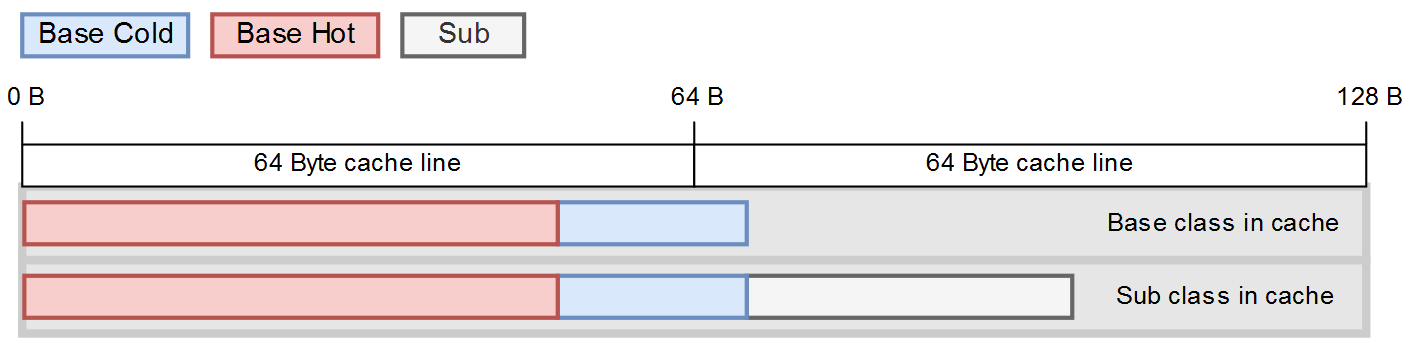
\includegraphics[width=0.83\textwidth,height=0.25\textwidth]{PICs/inheritance_split}
	\caption{Example of how a Base class and a Sub class could exist in the cache. In this case externalizing the Base's fields will effectively not reduce the Sub class' size enough to reduce the necessary amount of cache-lines to encompass it.}
	\label{inheritance_split}
\end{figure}
On the other hand, the split envisioned in \reffig{inheritance_split} would even separate the Sub class' fields over two cache-lines.\\\\
Not only there is the possibility to worsen the data layout for a sub-class by splitting its base, we might also end up splitting a sub-class yet after injecting the base classes' fields to it the changes are irrelevant as those new fields completely change the data layout once more \reffigp{inheritance_split_2}!
\begin{figure}[!htbp]
	\centering
	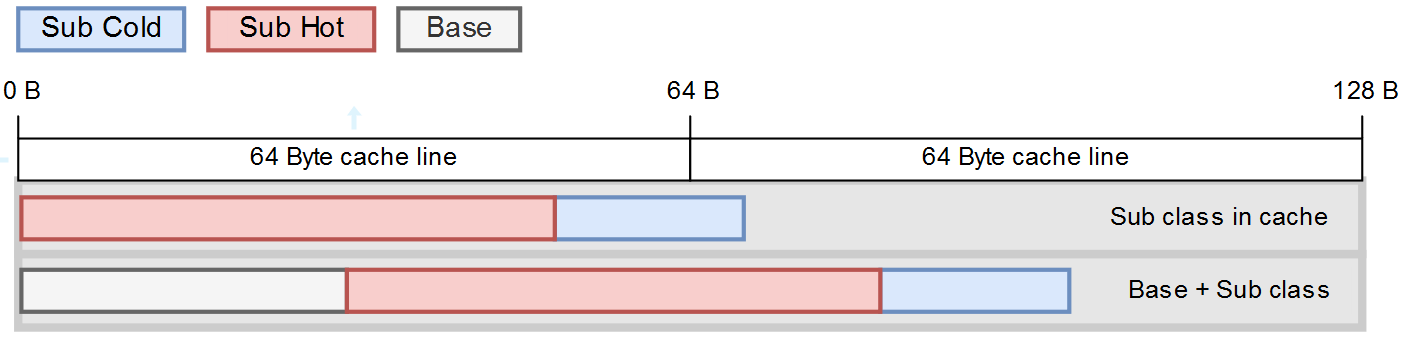
\includegraphics[width=0.83\textwidth,height=0.25\textwidth]{PICs/inheritance_split_2}
	\caption{Example of how a split in a sub class might be ineffective as soon, as its base's fields are brought into the picture.}
	\label{inheritance_split_2}
\end{figure}
Attributing members to sub-classes solves those issues relatively easily but splitting a record that is involved in inheritance becomes complex quite fast considering that a hierarchy might be arbitrarily large and especially when the language allows for multiple inheritance. When fields are attributed correctly we can reason about why certain fields should not be split (they have correlation). The next step would be for a Sub class to deem a base class' fields cold. This is a bold step, as the base class might actually rely on it quite frequently. Again this could be expressed by a cost-benefit estimation as we did before for the individual fields, when deciding whether to split it or not.\\\\
In case of a large inheritance hierarchy, instead of creating \textit{N} cold structs, we could instead merge them to one cold struct. This way when a record \textit{Sub} extends \textit{C}, which extends \textit{B}, which extends \textit{A}, The \textit{Sub} class would not end up having three cold struct pointers but one. Otherwise it would inherit it's bases' cold struct pointers as well\\\\
It is possible for automated Hot/Cold splits to comply with inheritance, however several factors need to be considered. A record's layout changes, as its bases change also structure padding and alignments will change as soon as a base changes. In order to correctly anticipate the data layout the inheritance hierarchy needs to be extracted and splits need to be executed in the correct order starting with the base classes so no changes to a record could result in consequent reevaluation of one of its sub classes.

\section{Conceptual limitations}
Until now we discussed issues, that for the most part can be solved applying further static analysis of the target source code. Unfortunately there are problems, that either partially invalidate our progress until now or plainly disallow COOP completely. This section will list several reasons to why COOP and this kind of optimization attempt is at least to be considered quite limited and actually to be precise not completely possible.
%\subsection{Static analysis on field usages using statistical means is dangerous}
%\subsection{Stand alone tool; Seamless integration into existing workspaces}
%In \refsec{motivation} we described easy integration into existing environments as an important presupposition for %its theoretical success. We decided against LLVM's optimization pass API so potential users would not depend on the %LLVM/Clang toolchain. COOP however still uses Clang as its interface to the target source code's AST and therefore %compiles the code using the Clang frontend. Accordingly COOP will not understand anything the Clang compiler doesn't %understand. While language specific keywords are defined in a standard, pragmas and attributes are not and differ %from compiler to compiler. 
\subsection{Templates}
A major drawback in source-to-source transformations is its inability (or limitation) to reason about and also change records, that include templated code. Templates are a useful feature, that allow for a program to interact with the compiler, that will transform it to machine code. Whenever a record contains a field of a templated/generic type our heuristic can't work as intended as it considers a fields type size to be relevant. A generic type does not have a defined type size in our static analysis.\\
This does not dismiss templated types altogether. As templates are resolved at compile time we could again do some of the compiler's job ourselves. While the Clang API will only find the generic templated version of a class definition for us, we could search for invocations of that class and retrieve template parameters to then construct the resulting class layout ourselves.\\
Our static analysis would then analyze all of the versions we can assemble for our templated record definition. However even though there will be different versions of that class definition in the end, source file transformations would affect all of the resulting versions. While our heuristics could find a good split in one version of it, another version might not benefit from that split.\\
As different versions of a templated record are determined at compile time we can retrieve all of the versions. There won't be unexpected 'new' versions of it being assembled at run-time. Only if each version of our templated definition profit from a split we could actually apply the respective changes.\\\\
While our source file changes limit us to consider all versions of a record an optimization performing on machine code or intermediate representations would actually have more optimization potential, as it could treat different versions differently.

\subsection{Data layout VS access patterns}
With the measurements we have seen, that an automatically improved data layout can result in better cache utilization and also performance, however it is bound to certain factors and conditions. The reasons for this we discussed in \refsec{dod}. Its all about data locality effective cache-line utilization and ultimately data throughput. Data is performance \mcp{nystrom}{272}. In \refsec{affect_on_data_layout} we elaborated on how our automated hot-cold split might be null and void the moment the target program allocates it's instances scattered on the heap and how COOP would therefore allocate contiguous blocks of memory to then redefine the allocations in the target code so our theoretically reduced stride would actually translate to real optimization.\\
That was one example of how theoretical improvement on the data layout might have been ineffective and luckily in this case there was a solution. However there is another dependency to our optimization, that can prevent COOP from actually accomplishing improvement. If the access patterns of the target program don't abide the best practices we talked about in \refsec{cdap} or if the program's task just does not depend on processing (iterating) its instances' members domain wise we again can't make use of reduced stride.\\
An improved data layout is a mighty tool only as long as the respective access patterns to it's instances allows for a minimized stride to result in improved cache-line utilization. It is therefore fairly easy to write a program, that will not profit from an 'improved' data layout and consequently not profit from COOP. In those cases the additional initialization overhead coming with our pool allocator will in most cases even result in deterioration of performance.

\subsection{Structural changes in record layouts}\label{scirl}
In \refsec{structure_padding_and_field_reordering} we explained why calculating a record's size in memory is not as easy as accumulating it's fields type sizes. Structure padding is done by the compiler to ensure optimal data loads. In order to determine, whether or not a split is beneficial we would calculate the original record's size including padding, to further reduce stride we would minimize padding by reordering the record's fields in a descending order.\\
This is a relatively trivial optimization, that depending on the original definition can have huge impacts on cache utilization for great amounts of data. In fact it is trivial enough to wonder why existing compilers don't do it.\\
Eric S. Raymond explains, that
\begin{quote}
	"\textit{Automatic reordering would interfere with a systems programmer’s ability to lay out structures that exactly match the byte and bit-level layout of memory-mapped device control blocks}" \mc{padding}.
\end{quote}
Other than that since we are altering an existing code base reordering fields has another implication. In \refsec{hidden_field_usages} we explained how field usages can stay undetected due to C/C++'s ability to manually create pointers. When given a source code there is always the possibility that for whatever reasons fields are accessed through pointers or even pointer arithmetic.
\begin{lstlisting}[language=C++, name={Simple example of why automated field rearrangements can't be considered legal.}, label={pointer_arithmetic_access}]
struct A{
	int a = 1;
	int b = 2;
} foo;
printf("%d\n", *(reinterpret_cast<int*>(&foo)+1)); //out: 2
\end{lstlisting}
\refcode{pointer_arithmetic_access} shows a simple example of how a record's field can be accessed without ever actually using it's identifier. Reordering fields inside a record would not break the target code, but induce bugs that are very hard to find and ultimately corrupt the semantic integrity of our 'optimized version'.\\
The follow up question is now: Why does COOP grant itself the liberty of reordering fields? The reason for this is that it already breaks code like \refcode{pointer_arithmetic_access} anyways, even without field rearrangements. COOP not only reorders fields it extracts them completely. Any pointer gymnastics, that would originally lead to a certain field can now no longer trust their record's data layout anyway. This is a conceptual contradiction to an optimization like ours and consequently invalidates COOP in its entirety! At least in terms of language compliance.\\\\
In conclusion an optimization process like COOP can only ever be executed in a reliable way when the user (or again further static analysis) can guarantee, that at no point in the target code base fields are accessed without invoking their identifiers.\\
Comparably harmless pointers hiding a field will corrupt the results of our metrics/heuristics and might lead to hazardous splits and deteriorated performance but pointer arithmetic and type punning might actually result in corrupted semantics.

\subsubsection{Implementation dependent layout specifics}
In addition to the previously mentioned concerns about structural changes in a record's layout it is also worth mentioning, that determining a record's size in Byte actually depends on the underlying language implementation.
In C the standard would not dictate the underlying type of an enum other than for it to be an integral type \mc{padding}. C++11 introduced typed enums. Untyped enums are guaranteed to be at least the size of an int. Also the position of virtual table pointers for dynamic dispatch varies depending on the compiler.
\begin{quote}
	"\textit{Traditionally, it was placed after the class's user-declared datamembers. However, some compilers have moved it to the beginning of the class for performance reasons.}" \mcp{kalev}{258}
\end{quote}
In fact the standard does not even demand dynamic dispatch to be implemented through virtual function tables and respective pointers.\\
Since our optimization operates in an environment where we can't use \textit{sizeof}, nor invoke the target compilers behavior right now it entirely depends on assumptions and common cases, for example dynamic dispatch being implemented through an external table of function pointers and the virtual table pointer being at the beginning of the class.\\
Since virtual table pointers are inherently 'hidden' members (added by the compiler like padding Bytes) we can't unintentionally rearrange them in terms of descending type size, however when determining a record's size they need to be considered, as they occupy memory on their own and might as well induce additional structure padding.\\
To properly adjust to these circumstances the user would need to be able to share information about the target compiler with COOP so it can invoke compiler dependent behavior and adjust certain routines.

%\subsection{Halting problem}
%can never analyze an algorithm reliably.

%\subsection{PGO/LTO}
%No static analysis!

\section{Conclusion}\label{conclusion}
In the evolution of modern hardware the memory units the memory components of our today's systems pose a bottleneck in terms of throughput. Caching mechanisms implemented in complex memory hierarchies provide measures to counter this performance discrepancy but their correct utilization is the programmer's responsibility.\\
Object Oriented Programming is a powerful paradigm that allows for a programmer to model a problem in concepts he or she is familiar with. It offers a mechanism of abstraction that is intuitively adapted to a variety of problems. While a programmer benefits from abstraction in terms of maintainability it usually translates to a data layout, that inefficiently utilizes our modern hardware.\\
Data oriented design practices focus on the problems data and pragmatically rationalizes abstraction in favor of locality principles. This may lead to code that is inferior in terms of maintainability but can and often will result in a performance boost as the resulting data layouts accommodate caching mechanisms better.\\
Automated support for DoD principles can be implemented in a languages compiler and seamlessly convert a record definition into a structure that abides locality principles. In C++ however there is no intrinsic support for such data structures. Template meta programming has the ability to interact with the compiler and can be used to introduce DoD support, it is however limited and leaves optimization responsibility to the programmer.\\
In an attempt to create a generic optimization pattern our exemplary implementation COOP parses a target set of source files and attempts to determine a record's fieldproperties. This enables us to execute an automated Hot/Cold split based on metrics and heuristics we tailored to identify cold fields. Changes in the target source code can in fact produce a semantic equivalent that bears the potential to utilize the cache better than the original.\\\\
Automated data layout optimizations bear high potential to move time consuming effort that requires a certain amount of knowledge and expertise from the programmer to an optimization tool. The programmer's responsibility to efficiently utilize the cache can effectively be transferred to a particular step in a build process. This saves time and reduces error potential. Most importantly with automated optimizations of this kind a programmer can maintain certain levels of abstraction which especially for novices will result in a more comfortable mindset while still profiting from superior cache utilization.\\\\
These optimizations are however highly dependent on a variety of factors. A multitude of programs and records disqualify as a subject to our optimization merely by not relying on common access patterns. Also programs that don't work with great sets of data will effectively not profit from an optimization that changes the data layout. There is a range of conceptual contradictions that either make a point against static analysis to determine split opportunities or source-to-source transformations as they rely on a target compiler's implementation specific behavior.\\\\
After having implemented and worked with an exemplary attempt to an automated optimization tool like COOP I am now positive, that static analysis to identify split opportunities is possible, however very limited in its precision and depends on a variety of factors. Future work on such analysis steps are possible however their effort is conceptually limited (see the halting problem) and compared to PGO probably not worth it. Complex and project contextual analyzes on an ASTs are very time consuming for big projects. In comparison I subjectively can't rate them superior to profile guided optimizations. On the one hand it is automated and therefore can be run over night, doesn't require supervision of a quality assurance team, but on the other hand since it tries to make educated guesses about run time specific behavior based on static data it will ultimately always include an error of unknown significance. In cases of low complexity and basic programming patterns that error might be small however as there are theoretically infinite scenarios a program can be constituted there is just no way of guaranteeing that a tool like COOP will always yield better results, than a split based on PGO data.\\
While I personally still support the idea of removing the programmer's responsibility to execute an optimization like a Hot/Cold split or transforming a record into AOSOA buckets, I can no longer endorse moving the responsibility from identifying split opportunities from the programmer to a tool that makes educated guesses.\\
It is perfectly possible to execute automated layout optimizations however the underlying information on which record/fields to split/externalize/turn into AOSOA should ideally be provided by the programmer. In this case for example a much better attempt at implementing COOP would be to either introduce an annotation that can mark a record/certain fields for a split or pass this information as command line parameters.\\
In order to comply with language features that resolve during compilation (like templated code) and to enable a tool like COOP to be integrated in an agile process it would also be advisable to move away from source-to-source transformations and instead execute LTOs (Link Time Optimization) or manually transform object files/executables. In case of LTOs we would need to develop compiler specific implementations. A more complex solution would only depend on the platform (\textit{exe, ELF}) and manipulate object files/executables directly. Denis Bakhvalov explained in a 2018 articel on \textit{Machine code layout optimizations} \mc{denis} how he automates function splitting, where he would extract cold code blocks from a function to new functions. Here code would be cold due to residing in a control flow statement that through profiling data cold be identified as rarely used. A similar project is Facebook's BOLT tool, that also operates on profiling data and modifies instruction placements in binaries. It is therefore independent of the compiler used to produce it \mc{bolt}.
